\documentclass[11pt,a4paper]{report}

% ─── Packages ───
\usepackage[utf8]{inputenc}
\usepackage[T1]{fontenc}
\usepackage[margin=1in, top=1.2in, bottom=1.2in]{geometry}
\usepackage{amsmath,amssymb,amsthm,mathtools}
\usepackage{xcolor}
\usepackage{titlesec}
\usepackage{titletoc}
\usepackage{fancyhdr}
\usepackage{enumitem}
\usepackage{tcolorbox}
\usepackage{booktabs}
\usepackage{graphicx}
\usepackage{hyperref}
\usepackage{cleveref}
\usepackage{tikz}
\usepackage{setspace}
\usepackage{parskip}
\usepackage{caption}
\usepackage{etoolbox}
\usepackage{array}
\usepackage{multirow}

\usetikzlibrary{arrows.meta, positioning, shapes.geometric, calc, decorations.pathmorphing, fit, backgrounds, chains, patterns}
\tcbuselibrary{skins,breakable,theorems}

% ─── Colors ───
\definecolor{darknavy}{HTML}{0d1b2a}
\definecolor{accentfire}{HTML}{e63946}
\definecolor{deepslate}{HTML}{1b263b}
\definecolor{softgold}{HTML}{c8a951}
\definecolor{darkbg}{HTML}{080e17}
\definecolor{sectionblue}{HTML}{1a3a5c}
\definecolor{subsecblue}{HTML}{2c5f8a}
\definecolor{defcolor}{HTML}{1565c0}
\definecolor{defbg}{HTML}{e3f2fd}
\definecolor{principlecolor}{HTML}{b71c1c}
\definecolor{principlebg}{HTML}{ffebee}
\definecolor{mechcolor}{HTML}{1b5e20}
\definecolor{mechbg}{HTML}{e8f5e9}
\definecolor{mathbg}{HTML}{f8f5ee}
\definecolor{notepurple}{HTML}{7b1fa2}
\definecolor{notebg}{HTML}{f3e5f5}
\definecolor{lightgray}{HTML}{f0f0f0}
\definecolor{darkgray}{HTML}{333333}
\definecolor{predcolor}{HTML}{e65100}
\definecolor{predbg}{HTML}{fff3e0}
\definecolor{compcolor}{HTML}{4a148c}
\definecolor{compbg}{HTML}{f3e5f5}
\definecolor{modelcolor}{HTML}{00695c}
\definecolor{modelbg}{HTML}{e0f2f1}
\definecolor{objcolor}{HTML}{880e4f}
\definecolor{objbg}{HTML}{fce4ec}
\definecolor{fepcolor}{HTML}{0d47a1}
\definecolor{fepbg}{HTML}{e3f2fd}

% ─── Hyperref Setup ───
\hypersetup{
    colorlinks=true,
    linkcolor=darknavy,
    citecolor=darknavy,
    urlcolor=deepslate,
    bookmarks=true,
    bookmarksnumbered=true,
    pdfauthor={Comprehensive Guide},
    pdftitle={Predictive Processing and Active Inference},
    pdfsubject={Consciousness, Free Energy Principle, Bayesian Brain, Active Inference},
}

% ─── Header/Footer ───
\pagestyle{fancy}
\fancyhf{}
\fancyhead[L]{\small\color{gray} Predictive Processing \& Active Inference}
\fancyhead[R]{\small\color{gray} Comprehensive Reading Material}
\fancyfoot[C]{\thepage}
\renewcommand{\headrulewidth}{0.4pt}
\renewcommand{\footrulewidth}{0pt}
\fancypagestyle{plain}{\fancyhf{}\fancyfoot[C]{\thepage}\renewcommand{\headrulewidth}{0pt}}

% ─── Chapter/Section Formatting ───
\titleformat{\chapter}[display]
  {\normalfont\huge\bfseries\color{darknavy}}
  {\chaptertitlename\ \thechapter}{20pt}{\Huge}
\titlespacing*{\chapter}{0pt}{-20pt}{30pt}
\titleformat{\section}{\normalfont\Large\bfseries\color{sectionblue}}{\thesection}{1em}{}
\titleformat{\subsection}{\normalfont\large\bfseries\color{subsecblue}}{\thesubsection}{1em}{}
\titleformat{\subsubsection}{\normalfont\normalsize\bfseries\color{darkgray}}{\thesubsubsection}{1em}{}

% ─── Tcolorbox environments ───
\newtcolorbox{principlebox}[1][]{enhanced, breakable, colback=principlebg, colframe=principlecolor, coltitle=white, fonttitle=\bfseries, title=#1, left=8pt, right=8pt, top=6pt, bottom=6pt, boxrule=0.5pt, arc=3pt, borderline west={3pt}{0pt}{principlecolor}, before skip=10pt, after skip=10pt}
\newtcolorbox{mechbox}[1][]{enhanced, breakable, colback=mechbg, colframe=mechcolor, coltitle=white, fonttitle=\bfseries, title=#1, left=8pt, right=8pt, top=6pt, bottom=6pt, boxrule=0.5pt, arc=3pt, borderline west={3pt}{0pt}{mechcolor}, before skip=10pt, after skip=10pt}
\newtcolorbox{definitionbox}[1][]{enhanced, breakable, colback=defbg, colframe=defcolor, coltitle=white, fonttitle=\bfseries, title=#1, left=8pt, right=8pt, top=6pt, bottom=6pt, boxrule=0.5pt, arc=3pt, borderline west={3pt}{0pt}{defcolor}, before skip=10pt, after skip=10pt}
\newtcolorbox{mathbox}{enhanced, colback=mathbg, colframe=mathbg!70!black, left=8pt, right=8pt, top=6pt, bottom=6pt, boxrule=0.3pt, arc=2pt, before skip=8pt, after skip=8pt}
\newtcolorbox{notebox}[1][Note]{enhanced, breakable, colback=notebg, colframe=notepurple, coltitle=white, fonttitle=\bfseries, title=#1, left=8pt, right=8pt, top=6pt, bottom=6pt, boxrule=0.5pt, arc=3pt, borderline west={3pt}{0pt}{notepurple}, before skip=10pt, after skip=10pt}
\newtcolorbox{predbox}[1][]{enhanced, breakable, colback=predbg, colframe=predcolor, coltitle=white, fonttitle=\bfseries, title=#1, left=8pt, right=8pt, top=6pt, bottom=6pt, boxrule=0.5pt, arc=3pt, borderline west={3pt}{0pt}{predcolor}, before skip=10pt, after skip=10pt}
\newtcolorbox{compbox}[1][]{enhanced, breakable, colback=compbg, colframe=compcolor, coltitle=white, fonttitle=\bfseries, title=#1, left=8pt, right=8pt, top=6pt, bottom=6pt, boxrule=0.5pt, arc=3pt, borderline west={3pt}{0pt}{compcolor}, before skip=10pt, after skip=10pt}
\newtcolorbox{modelbox}[1][]{enhanced, breakable, colback=modelbg, colframe=modelcolor, coltitle=white, fonttitle=\bfseries, title=#1, left=8pt, right=8pt, top=6pt, bottom=6pt, boxrule=0.5pt, arc=3pt, borderline west={3pt}{0pt}{modelcolor}, before skip=10pt, after skip=10pt}
\newtcolorbox{objbox}[1][]{enhanced, breakable, colback=objbg, colframe=objcolor, coltitle=white, fonttitle=\bfseries, title=#1, left=8pt, right=8pt, top=6pt, bottom=6pt, boxrule=0.5pt, arc=3pt, borderline west={3pt}{0pt}{objcolor}, before skip=10pt, after skip=10pt}
\newtcolorbox{fepbox}[1][]{enhanced, breakable, colback=fepbg, colframe=fepcolor, coltitle=white, fonttitle=\bfseries, title=#1, left=8pt, right=8pt, top=6pt, bottom=6pt, boxrule=0.5pt, arc=3pt, borderline west={3pt}{0pt}{fepcolor}, before skip=10pt, after skip=10pt}
\newtcolorbox{examplebox}[1][Example]{enhanced, breakable, colback=lightgray, colframe=darknavy!60, coltitle=white, fonttitle=\bfseries, title=#1, left=8pt, right=8pt, top=6pt, bottom=6pt, boxrule=0.5pt, arc=3pt, before skip=10pt, after skip=10pt}

\setlength{\parindent}{0pt}
\setlength{\parskip}{6pt}

% ══════════════════════════════════════════════════════════════
\begin{document}

% ─── COVER PAGE ───
\begin{titlepage}
\begin{tikzpicture}[remember picture, overlay]
  \fill[darkbg] (current page.south west) rectangle (current page.north east);
  \fill[accentfire] ([yshift=-11cm]current page.north west) rectangle ([yshift=-10.85cm]current page.north east);
  % Decorative: hierarchical prediction arrows
  \foreach \y/\op in {-12/0.06, -13.5/0.08, -15/0.10, -16.5/0.08} {
    \draw[accentfire, opacity=\op, line width=0.8pt, -Stealth] (3, \y) -- (6, \y);
    \draw[white, opacity=\op, line width=0.5pt, -Stealth, dashed] (6, \y+0.3) -- (3, \y+0.3);
  }
  \node[text=white, opacity=0.04, font=\scriptsize, rotate=90] at (2.3, -14.2) {prediction error};
  \node[text=accentfire, opacity=0.04, font=\scriptsize, rotate=90] at (6.7, -14.2) {predictions};
  % Markov blanket sketch
  \draw[accentfire, opacity=0.06, line width=0.5pt, dashed] (8,-13) ellipse (1.5 and 2.5);
  \draw[white, opacity=0.04, line width=0.5pt] (8,-13) ellipse (0.8 and 1.5);
  \node[text=accentfire, opacity=0.04, scale=16] at ([yshift=-4cm, xshift=5cm]current page.center) {\textbf{FE}};
\end{tikzpicture}

\vspace*{4cm}
\begin{center}
  {\fontsize{32}{40}\selectfont\bfseries\color{white} Predictive Processing\\[8pt] \& Active Inference}\\[24pt]
  {\Large\color{gray!70} A Comprehensive Mathematical \& Conceptual Guide}\\[20pt]
  {\color{accentfire}\rule{6cm}{1pt}}\\[20pt]
  {\large\color{gray!60} The Free Energy Principle, the Bayesian Brain,\\[4pt] and Consciousness as Controlled Hallucination}\\[40pt]
  {\color{softgold}\large Friston $\bullet$ Clark $\bullet$ Hohwy $\bullet$ Seth}\\[8pt]
  {\color{gray!50}\normalsize Free Energy $\bullet$ Generative Models $\bullet$ Markov Blankets $\bullet$ Precision $\bullet$ Selfhood}\\[60pt]
  {\color{gray!40}\small Comprehensive Study Material \quad$\vert$\quad February 2026}
\end{center}
\end{titlepage}

% ─── TABLE OF CONTENTS ───
\tableofcontents
\thispagestyle{plain}
\newpage


% ══════════════════════════════════════════════════════════════
\chapter{Introduction to Predictive Processing}
% ══════════════════════════════════════════════════════════════

\section{What is Predictive Processing?}

\textbf{Predictive Processing} (PP) is a theoretical framework proposing that the brain is fundamentally a \textbf{prediction machine}. Rather than passively receiving and processing sensory input bottom-up, the brain actively generates \textbf{top-down predictions} about what it expects to sense, and then compares these predictions with actual sensory input. The difference---the \textbf{prediction error}---drives learning, perception, and action.

\begin{definitionbox}[Core Claim of Predictive Processing]
The brain maintains a \textbf{generative model} of the world---a hierarchical, probabilistic model that generates predictions about sensory input at every level of the cortical hierarchy. Perception is not a passive reading of sensory data but a process of \textbf{Bayesian inference}: the brain infers the most probable causes of its sensory signals by iteratively updating its generative model to minimize \textbf{prediction error}. Consciousness arises from the brain's ``best guess'' about the hidden causes of its sensations.
\end{definitionbox}

The framework has several names and formulations:
\begin{itemize}[leftmargin=1.5em]
  \item \textbf{Predictive Processing / Predictive Coding} (Rao \& Ballard, 1999; Friston, 2005)
  \item \textbf{The Free Energy Principle} (FEP) (Friston, 2006, 2010): A mathematical framework grounding PP in variational inference and information theory.
  \item \textbf{Active Inference} (Friston, 2009): The extension of PP to action, where organisms act on the world to fulfill their predictions.
  \item \textbf{The Bayesian Brain Hypothesis} (Knill \& Pouget, 2004): The broader claim that neural computation implements Bayesian inference.
  \item \textbf{Controlled Hallucination} (Seth, 2021): A vivid description of PP's view of conscious perception.
\end{itemize}

\section{Historical Context}

\subsection{Helmholtz and Unconscious Inference}

The idea that perception involves inference dates to \textbf{Hermann von Helmholtz} (1867), who proposed that the brain performs ``unconscious inferences'' to interpret ambiguous sensory data. Helmholtz recognized that the retinal image is inherently ambiguous (multiple 3D scenes can produce the same 2D image) and that the brain must use prior knowledge to resolve this ambiguity.

\subsection{The Computational Turn}

In the late 20th century, several streams converged:
\begin{itemize}[leftmargin=1.5em]
  \item \textbf{Bayesian statistics:} Formalized the combination of prior knowledge with new evidence.
  \item \textbf{Machine learning:} Generative models, variational methods, and hierarchical Bayesian models provided computational tools.
  \item \textbf{Neuroscience:} Discovery of massive feedback connections in cortex (feedback outnumbers feedforward $\sim$10:1 in many areas) demanded explanation.
  \item \textbf{Rao \& Ballard (1999):} Demonstrated that predictive coding could explain extra-classical receptive field properties in V1 using a hierarchical model.
\end{itemize}

\subsection{Friston and the Free Energy Principle}

\textbf{Karl Friston} (University College London) unified these ideas under the \textbf{Free Energy Principle} (FEP), arguing that all adaptive behavior---perception, action, learning, development, evolution---can be understood as minimizing a single quantity: \textbf{variational free energy}. This transformed PP from a model of perception into a unified theory of brain function and, potentially, consciousness.

\section{Overview of the Framework}

\begin{enumerate}[leftmargin=2em]
  \item \textbf{Generative model:} The brain encodes a hierarchical, probabilistic model of the causal structure of the world.
  \item \textbf{Prediction:} Each level of the hierarchy generates predictions about the level below.
  \item \textbf{Prediction error:} The difference between prediction and actual input is computed and propagated upward.
  \item \textbf{Inference:} The brain minimizes prediction error by updating its model (perception) or by acting on the world (action).
  \item \textbf{Precision:} The brain estimates the reliability (precision) of its predictions and prediction errors, and weights them accordingly (attention).
  \item \textbf{Consciousness:} Arises from the content of the generative model---the brain's ``best guess'' about the world and itself.
\end{enumerate}


% ══════════════════════════════════════════════════════════════
\chapter{Mathematical Foundations}
% ══════════════════════════════════════════════════════════════

This chapter develops the mathematical apparatus underlying PP and the Free Energy Principle. The formalism is essential for understanding the theory's explanatory power and its connection to consciousness.

\section{Bayesian Inference}

PP is fundamentally Bayesian. Given observed data $\mathbf{y}$ and hidden causes $\boldsymbol{\theta}$:

\begin{mathbox}
\vspace{-6pt}
\textbf{Bayes' theorem:}
\[
  \underbrace{p(\boldsymbol{\theta} \mid \mathbf{y})}_{\text{posterior}} = \frac{\overbrace{p(\mathbf{y} \mid \boldsymbol{\theta})}^{\text{likelihood}} \;\cdot\; \overbrace{p(\boldsymbol{\theta})}^{\text{prior}}}{\underbrace{p(\mathbf{y})}_{\text{evidence (marginal likelihood)}}}
\]
\vspace{-8pt}
\end{mathbox}

\begin{itemize}[leftmargin=1.5em]
  \item \textbf{Prior} $p(\boldsymbol{\theta})$: The brain's existing beliefs about the world before observing data.
  \item \textbf{Likelihood} $p(\mathbf{y} \mid \boldsymbol{\theta})$: How probable the sensory data are given a particular state of the world.
  \item \textbf{Posterior} $p(\boldsymbol{\theta} \mid \mathbf{y})$: The updated belief after incorporating the data.
  \item \textbf{Evidence} $p(\mathbf{y})$: The total probability of the data under the model (a normalizing constant).
\end{itemize}

\textbf{Perception} in PP is the process of computing (or approximating) the posterior $p(\boldsymbol{\theta} \mid \mathbf{y})$. The conscious percept corresponds to the posterior mode or mean---the brain's best estimate of the world's hidden causes.

\section{The Problem of Intractability}

Computing the exact posterior requires evaluating the evidence:
\[
  p(\mathbf{y}) = \int p(\mathbf{y} \mid \boldsymbol{\theta})\, p(\boldsymbol{\theta})\, d\boldsymbol{\theta}
\]

For realistic generative models, this integral is \textbf{intractable}---it cannot be computed exactly because it involves summing over an astronomically large space of hidden causes. The brain must therefore use \emph{approximate} inference.

\section{Variational Inference}

The Free Energy Principle uses \textbf{variational inference} to approximate the intractable posterior. The idea: instead of computing $p(\boldsymbol{\theta} \mid \mathbf{y})$ directly, find an approximate distribution $q(\boldsymbol{\theta})$ from a tractable family that is as close as possible to the true posterior.

\begin{definitionbox}[Variational Free Energy]
The \textbf{variational free energy} $F$ is defined as:
\begin{align}
  F &= \underbrace{D_{\mathrm{KL}}\!\left[q(\boldsymbol{\theta}) \;\|\; p(\boldsymbol{\theta} \mid \mathbf{y})\right]}_{\geq\, 0\; \text{(KL divergence)}} \;-\; \underbrace{\ln p(\mathbf{y})}_{\text{log evidence}} \label{eq:fe_def}
\end{align}
Rearranging:
\begin{align}
  F &= \underbrace{-\mathbb{E}_{q}\!\left[\ln p(\mathbf{y} \mid \boldsymbol{\theta})\right]}_{\text{expected energy (prediction error)}} + \underbrace{D_{\mathrm{KL}}\!\left[q(\boldsymbol{\theta}) \;\|\; p(\boldsymbol{\theta})\right]}_{\text{complexity (deviation from prior)}} \label{eq:fe_decomp}
\end{align}
Equivalently:
\begin{align}
  F &= -\underbrace{\mathbb{E}_{q}\!\left[\ln p(\mathbf{y}, \boldsymbol{\theta})\right]}_{\text{expected log joint}} + \underbrace{\mathbb{E}_{q}\!\left[\ln q(\boldsymbol{\theta})\right]}_{\text{negative entropy of }q} \label{eq:fe_alt}
\end{align}
\end{definitionbox}

\begin{principlebox}[Key Properties of Free Energy]
\begin{enumerate}[leftmargin=1.5em]
  \item $F \geq -\ln p(\mathbf{y})$. Free energy is an \textbf{upper bound} on surprise (negative log evidence). Minimizing $F$ is equivalent to maximizing a lower bound on the evidence (the ELBO).
  \item When $q(\boldsymbol{\theta}) = p(\boldsymbol{\theta} \mid \mathbf{y})$ (the approximate equals the true posterior), the KL divergence is zero and $F = -\ln p(\mathbf{y})$ exactly.
  \item Minimizing $F$ with respect to $q$ performs \textbf{approximate Bayesian inference}: it brings $q$ closer to the true posterior.
  \item Minimizing $F$ with respect to model parameters performs \textbf{learning}: it improves the generative model.
  \item Minimizing $F$ with respect to \textbf{actions} performs \textbf{active inference}: it changes sensory input to match predictions.
\end{enumerate}
\end{principlebox}

\section{The Generative Model}

At the heart of PP is a \textbf{hierarchical generative model} that specifies how hidden causes generate sensory observations.

\begin{definitionbox}[Hierarchical Generative Model]
A generative model consists of:
\begin{align}
  \text{Observation model:}\quad \mathbf{y} &= g_0(\mathbf{x}_1) + \boldsymbol{\varepsilon}_0, \qquad \boldsymbol{\varepsilon}_0 \sim \mathcal{N}(0, \Pi_0^{-1}) \label{eq:obs_model}\\[4pt]
  \text{Level } l \text{ dynamics:}\quad \mathbf{x}_l &= g_l(\mathbf{x}_{l+1}) + \boldsymbol{\varepsilon}_l, \qquad \boldsymbol{\varepsilon}_l \sim \mathcal{N}(0, \Pi_l^{-1}) \label{eq:level_l}\\[4pt]
  \text{Top-level prior:}\quad \mathbf{x}_L &\sim p(\mathbf{x}_L) \label{eq:top_prior}
\end{align}
where $\mathbf{x}_l$ are hidden states at level $l$, $g_l$ are nonlinear generative functions mapping higher levels to lower, $\boldsymbol{\varepsilon}_l$ are prediction errors (Gaussian noise), and $\Pi_l$ are \textbf{precision matrices} (inverse covariance) encoding the reliability of predictions at each level.
\end{definitionbox}

The generative model specifies how the brain believes the world works: high-level causes ($\mathbf{x}_L$: objects, scenes, agents) generate intermediate representations ($\mathbf{x}_{l}$: surfaces, edges, motion) which generate sensory data ($\mathbf{y}$: retinal images, cochlear signals).

\section{Predictive Coding: Message Passing}

\textbf{Predictive coding} implements variational inference in the hierarchical model through local message passing between cortical levels. At each level $l$:

\begin{fepbox}[Predictive Coding Update Equations]
\textbf{Prediction error:}
\begin{align}
  \boldsymbol{\varepsilon}_l &= \mathbf{x}_l - g_l(\hat{\mathbf{x}}_{l+1}) \label{eq:pe}
\end{align}
\textbf{State update (gradient descent on free energy):}
\begin{align}
  \dot{\hat{\mathbf{x}}}_{l} &= D\hat{\mathbf{x}}_{l} + \underbrace{\frac{\partial g_{l-1}^T}{\partial \hat{\mathbf{x}}_l}\, \Pi_{l-1}\, \boldsymbol{\varepsilon}_{l-1}}_{\text{bottom-up: prediction error from below}} - \underbrace{\Pi_l\, \boldsymbol{\varepsilon}_l}_{\text{top-down: prediction error at this level}} \label{eq:state_update}
\end{align}
\textbf{Precision update:}
\begin{align}
  \dot{\hat{\Pi}}_l &\propto -\frac{\partial F}{\partial \hat{\Pi}_l} = \frac{1}{2}\left(\hat{\Pi}_l^{-1} - \boldsymbol{\varepsilon}_l \boldsymbol{\varepsilon}_l^T\right) \label{eq:prec_update}
\end{align}
\end{fepbox}

\textbf{Neural interpretation:}
\begin{itemize}[leftmargin=1.5em]
  \item $\hat{\mathbf{x}}_l$: activity of \textbf{representation units} (deep-layer pyramidal neurons) encoding the estimated state.
  \item $\boldsymbol{\varepsilon}_l$: activity of \textbf{prediction error units} (superficial-layer pyramidal neurons).
  \item $g_l(\hat{\mathbf{x}}_{l+1})$: \textbf{feedback (top-down) predictions} sent from level $l{+}1$.
  \item $\Pi_l \boldsymbol{\varepsilon}_l$: \textbf{precision-weighted prediction error} sent feedforward to level $l{+}1$.
  \item Feedforward signals carry prediction errors; feedback signals carry predictions.
\end{itemize}

\section{Precision and Attention}

\textbf{Precision} $\Pi_l$ is the inverse variance of prediction errors at level $l$. It encodes the \textbf{reliability} or \textbf{confidence} in signals:

\begin{mathbox}
\vspace{-6pt}
\[
  \text{Precision-weighted prediction error:}\quad \xi_l = \Pi_l\, \boldsymbol{\varepsilon}_l
\]
High precision $\Pi_l$ means prediction errors at level $l$ are trusted and given high weight. Low precision means they are unreliable and down-weighted.
\vspace{-4pt}
\end{mathbox}

\begin{principlebox}[Precision $\equiv$ Attention]
In PP, \textbf{attention} is the optimization of precision. Attending to a stimulus means increasing the precision (gain) of prediction errors arising from that stimulus, so they have more influence on the posterior estimate. This connects directly to gain modulation in neural circuits:
\[
  \text{Attention to level } l \;\equiv\; \text{increasing } \Pi_l \;\equiv\; \text{amplifying prediction errors at level } l
\]
This provides a principled, mathematically grounded account of attention within the PP framework.
\end{principlebox}


% ══════════════════════════════════════════════════════════════
\chapter{The Free Energy Principle}
% ══════════════════════════════════════════════════════════════

\section{From Predictive Coding to Universal Principle}

Karl Friston elevated predictive coding from a model of perception to a \textbf{universal principle of self-organizing systems}. The Free Energy Principle (FEP) states:

\begin{fepbox}[The Free Energy Principle]
Any self-organizing system that maintains its structural and functional integrity must minimize its \textbf{variational free energy}. This is equivalent to:
\begin{enumerate}[leftmargin=1.5em]
  \item Minimizing \textbf{surprise} (negative log evidence) about sensory states
  \item Maximizing the \textbf{evidence} for the system's generative model of the world
  \item Performing approximate \textbf{Bayesian inference} on the causes of sensory input
  \item Maintaining the system within a bounded set of states (its ``attracting set'')
\end{enumerate}
Formally: biological systems minimize $F = \mathbb{E}_q[\ln q(\boldsymbol{\theta}) - \ln p(\mathbf{y}, \boldsymbol{\theta})]$.
\end{fepbox}

\section{Markov Blankets}

A central concept in the FEP is the \textbf{Markov blanket}:

\begin{definitionbox}[Markov Blanket]
A \textbf{Markov blanket} of a set of states $\boldsymbol{\mu}$ (internal states) is the set of states $\mathbf{b}$ that separates $\boldsymbol{\mu}$ from everything else (external states $\boldsymbol{\eta}$), such that $\boldsymbol{\mu}$ and $\boldsymbol{\eta}$ are conditionally independent given $\mathbf{b}$:
\[
  p(\boldsymbol{\mu}, \boldsymbol{\eta} \mid \mathbf{b}) = p(\boldsymbol{\mu} \mid \mathbf{b})\, p(\boldsymbol{\eta} \mid \mathbf{b})
\]
The blanket is partitioned into \textbf{sensory states} $\mathbf{s}$ (influenced by external states) and \textbf{active states} $\mathbf{a}$ (influencing external states):
\[
  \mathbf{b} = (\mathbf{s}, \mathbf{a})
\]
\end{definitionbox}

\begin{center}
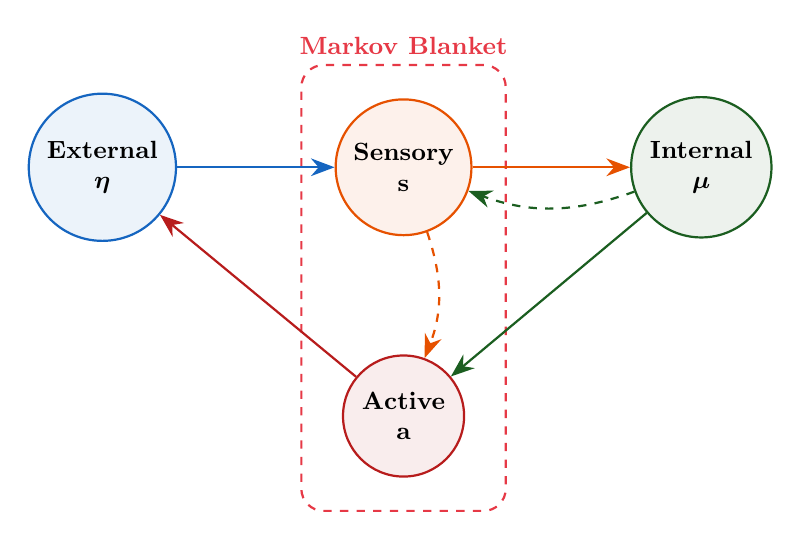
\begin{tikzpicture}[
    state/.style={circle, draw=#1, fill=#1!8, thick, minimum size=1.5cm, font=\small\bfseries, align=center},
    arr/.style={-{Stealth[length=3mm]}, thick, #1},
    node distance=2.5cm,
  ]
  \node[state=defcolor] (ext) {External\\$\boldsymbol{\eta}$};
  \node[state=predcolor, right=2cm of ext] (s) {Sensory\\$\mathbf{s}$};
  \node[state=mechcolor, right=2cm of s] (int) {Internal\\$\boldsymbol{\mu}$};
  \node[state=principlecolor, below=1.5cm of s] (a) {Active\\$\mathbf{a}$};

  \draw[arr=defcolor] (ext) -- (s);
  \draw[arr=predcolor] (s) -- (int);
  \draw[arr=mechcolor] (int) -- (a);
  \draw[arr=principlecolor] (a) -- (ext);
  \draw[arr=mechcolor, dashed] (int) to[bend left=20] (s);
  \draw[arr=predcolor, dashed] (s) to[bend left=20] (a);

  % Blanket boundary
  \begin{scope}[on background layer]
    \node[draw=accentfire, dashed, thick, rounded corners=8pt, fit=(s)(a), inner sep=12pt, label={[text=accentfire, font=\small\bfseries]above:Markov Blanket}] {};
  \end{scope}
\end{tikzpicture}
\end{center}
\vspace{-2pt}
{\small\centering\textit{Figure: Markov blanket separating internal states from external states. Sensory states mediate inward influence; active states mediate outward influence.}\par}

For a brain: external states are the world; sensory states are receptor activations; active states are motor commands; internal states are neural activity encoding beliefs about the world.

\section{Surprise and Self-Evidencing}

The FEP can be understood through the concept of \textbf{surprise} (or \textbf{surprisal}):

\begin{mathbox}
\vspace{-8pt}
\[
  \text{Surprise:}\quad \mathfrak{S}(\mathbf{y}) = -\ln p(\mathbf{y} \mid m)
\]
where $m$ is the organism's generative model. High surprise means the sensory input was unexpected under the model. The free energy $F \geq \mathfrak{S}$ provides an upper bound on surprise.
\vspace{-4pt}
\end{mathbox}

An organism that minimizes free energy over time will, on average, occupy states with low surprise---states that are expected under its model. Since the model encodes the organism's ``preferred'' states (e.g., a fish expects to be in water, at a certain temperature, etc.), minimizing surprise is equivalent to maintaining the organism within its viable states. Friston calls this \textbf{self-evidencing}: the organism provides evidence for its own model of existence.

\section{Active Inference}

The FEP extends to action through \textbf{active inference}: instead of only updating beliefs to match sensory input (perception), the organism can also change the world to match its predictions (action).

\begin{fepbox}[Active Inference]
Free energy can be minimized in two ways:
\begin{enumerate}[leftmargin=1.5em]
  \item \textbf{Perceptual inference:} Update internal states $\boldsymbol{\mu}$ (beliefs) to better predict sensory input:
  \[
    \dot{\boldsymbol{\mu}} = -\frac{\partial F}{\partial \boldsymbol{\mu}} \quad\text{(gradient descent on } F \text{ w.r.t.\ beliefs)}
  \]
  \item \textbf{Active inference:} Update active states $\mathbf{a}$ (actions) to change sensory input to match predictions:
  \[
    \dot{\mathbf{a}} = -\frac{\partial F}{\partial \mathbf{a}} = -\frac{\partial \mathbf{y}}{\partial \mathbf{a}} \cdot \frac{\partial F}{\partial \mathbf{y}} \quad\text{(gradient descent on } F \text{ w.r.t.\ actions)}
  \]
\end{enumerate}
Action is driven by the same quantity as perception---prediction error---but instead of updating the model, it changes the world.
\end{fepbox}

\begin{examplebox}[Active Inference: Picking Up a Cup]
You predict the sensation of holding a cup (proprioceptive predictions of arm position, tactile predictions of cup contact). The prediction error (arm is not yet holding cup) drives motor commands that move the arm to grasp the cup. When the cup is grasped, prediction errors are minimized. You did not need a separate ``motor plan''---the predictions themselves drive action.
\end{examplebox}

\section{Expected Free Energy and Planning}

For planning and decision-making, active inference uses \textbf{expected free energy} $G$:

\begin{mathbox}
\vspace{-6pt}
\[
  G(\pi) = \underbrace{\mathbb{E}_{q}\!\left[D_{\mathrm{KL}}\!\left[q(\boldsymbol{\theta} \mid \mathbf{y}_\pi) \;\|\; q(\boldsymbol{\theta})\right]\right]}_{\text{epistemic value (information gain)}} + \underbrace{\mathbb{E}_{q}\!\left[-\ln p(\mathbf{y}_\pi)\right]}_{\text{pragmatic value (expected surprise)}}
\]
\vspace{-8pt}
\end{mathbox}

where $\pi$ denotes a policy (sequence of actions) and $\mathbf{y}_\pi$ denotes the predicted sensory outcomes under policy $\pi$. The brain selects the policy $\pi^*$ that minimizes expected free energy:
\[
  \pi^* = \arg\min_\pi G(\pi)
\]

This decomposes into two drives: \textbf{epistemic value} (seeking information, resolving uncertainty) and \textbf{pragmatic value} (achieving preferred outcomes). The balance between exploration and exploitation emerges naturally.


% ══════════════════════════════════════════════════════════════
\chapter{Hierarchical Predictive Coding in the Brain}
% ══════════════════════════════════════════════════════════════

\section{Cortical Microcircuit Architecture}

Predictive coding maps naturally onto the \textbf{laminar structure} of cortex:

\begin{mechbox}[Cortical Implementation of Predictive Coding]
\begin{itemize}[leftmargin=1.5em]
  \item \textbf{Deep pyramidal neurons} (layers 5/6): Encode expectations $\hat{\mathbf{x}}_l$ (representation units). Send top-down predictions via feedback connections to the level below.
  \item \textbf{Superficial pyramidal neurons} (layer 2/3): Compute and encode prediction errors $\boldsymbol{\varepsilon}_l$. Send prediction errors feedforward to the level above.
  \item \textbf{Inhibitory interneurons} (layers 2/3, 4): Mediate the subtraction operation (actual input minus prediction) and regulate gain (precision).
  \item \textbf{Feedback connections} (layers 5/6 $\to$ layers 1, 5/6): Carry predictions from higher to lower areas.
  \item \textbf{Feedforward connections} (layer 2/3 $\to$ layer 4): Carry prediction errors from lower to higher areas.
\end{itemize}
\end{mechbox}

\section{Oscillatory Signatures}

Predictive coding maps onto specific oscillatory frequency bands:

\begin{center}
\renewcommand{\arraystretch}{1.3}
\begin{tabular}{>{\raggedright}p{3.5cm} >{\raggedright}p{3cm} >{\raggedright\arraybackslash}p{6cm}}
  \toprule
  \textbf{Signal} & \textbf{Frequency Band} & \textbf{Function in PP} \\
  \midrule
  Predictions (top-down) & Alpha/beta (8--30 Hz) & Carry predictions from higher to lower areas \\
  Prediction errors (bottom-up) & Gamma ($>$30 Hz) & Carry precision-weighted errors upward \\
  Precision modulation & Alpha (8--13 Hz) & Inhibitory gating; low alpha = high precision \\
  Cross-frequency coupling & Theta-gamma nesting & Temporal coordination of hierarchical inference \\
  \bottomrule
\end{tabular}
\end{center}

This pattern---gamma for feedforward prediction errors, alpha/beta for feedback predictions---has been confirmed by van Kerkoerle et al.\ (2014) and Bastos et al.\ (2015), as discussed in the RPT chapter.

\section{Empirical Evidence for Predictive Coding}

\subsection{Mismatch Negativity (MMN)}

The \textbf{mismatch negativity} is an event-related potential ($\sim$100--250 ms) generated when an auditory stimulus violates a regular pattern (e.g., an occasional deviant tone in a sequence of standard tones). PP explains MMN directly: the brain builds a predictive model of the auditory sequence; the deviant triggers a large prediction error.

The MMN amplitude scales with the \textbf{precision-weighted prediction error}---deviants that are more surprising (less expected) or more reliable (in quiet conditions) produce larger MMN.

\subsection{Repetition Suppression and Expectation Suppression}

\textbf{Repetition suppression:} Repeated stimuli evoke progressively weaker neural responses. PP interpretation: the generative model learns to predict the repeated stimulus, reducing prediction error.

\textbf{Expectation suppression:} Expected stimuli (even novel ones) evoke weaker responses than unexpected stimuli. PP interpretation: prediction errors are small when the stimulus matches the model's prediction.

\subsection{Perceptual Illusions}

PP naturally explains illusions as cases where the generative model's prior dominates over weak sensory evidence:

\begin{examplebox}[The Hollow Mask Illusion]
A hollow (concave) face mask appears convex---the brain ``sees'' a normal face. PP explanation: the prior for faces (faces are convex) is so strong that it overrides the (relatively weak) sensory evidence for concavity. The generative model's prediction (convex face) wins over the data.
\end{examplebox}

This illusion is disrupted in schizophrenia---consistent with the hypothesis that schizophrenia involves weakened priors (see Section 5.4).


% ══════════════════════════════════════════════════════════════
\chapter{Consciousness in Predictive Processing}
% ══════════════════════════════════════════════════════════════

PP is not a theory of consciousness per se, but several researchers have developed explicit accounts of consciousness within the PP framework.

\section{Consciousness as the Content of the Generative Model}

The simplest PP account: \textbf{conscious experience is the content of the brain's generative model}---the posterior estimate $\hat{\mathbf{x}}$ at all levels of the hierarchy.

\begin{principlebox}[Consciousness as Bayesian Best Guess]
What we consciously experience is not the raw sensory data $\mathbf{y}$, but the brain's \textbf{posterior estimate} of the hidden causes of that data:
\[
  \text{Conscious percept} \approx \hat{\mathbf{x}} = \arg\max_{\mathbf{x}}\; p(\mathbf{x} \mid \mathbf{y}) \approx \arg\min_{\mathbf{x}}\; F(\mathbf{x}, \mathbf{y})
\]
Perception is a ``controlled hallucination'': the brain generates a model of the world and constrains it with sensory data. What we see, hear, and feel is the model's output, not the data itself.
\end{principlebox}

\subsection{``Controlled Hallucination'' (Anil Seth)}

\textbf{Anil Seth} (University of Sussex) has developed the most vivid characterization: conscious perception is a \textbf{controlled hallucination}. The brain is always hallucinating---generating a model of the world from the top down. Sensory data merely \emph{constrains} the hallucination, keeping it consistent with reality.

When the hallucination is well-constrained by data, we call it ``perception.'' When it is poorly constrained (as in dreaming, psychedelics, or psychosis), the hallucination becomes more vivid, bizarre, or dissociated from reality.

\section{Seth's ``Beast Machine'' Framework}

Seth (2021) extends the PP account specifically to consciousness, proposing:

\begin{modelbox}[Seth's Predictive Processing Account of Consciousness]
\begin{enumerate}[leftmargin=1.5em]
  \item \textbf{Perceptual consciousness} = the content of the generative model's posterior estimates about the external world (colors, shapes, sounds).
  \item \textbf{Self-consciousness / embodied selfhood} = the content of the generative model's posterior estimates about the \emph{body} (interoception, proprioception, agency).
  \item \textbf{Emotional experience} = precision-weighted interoceptive prediction errors integrated with allostatic regulation.
  \item \textbf{The ``real problem'' of consciousness:} Rather than asking \emph{why} there is experience (the Hard Problem), Seth proposes the \emph{real problem}: explaining the specific character and structure of experience in terms of generative models.
\end{enumerate}
\end{modelbox}

\section{Precision, Attention, and the ``Level'' of Consciousness}

A key PP contribution is the account of how the \textbf{level} (quantity) of consciousness relates to precision:

\begin{mathbox}
\vspace{-6pt}
The overall ``level'' of consciousness $\mathcal{L}$ may be related to the total precision-weighted prediction error across the hierarchy:
\[
  \mathcal{L} \propto \sum_l \text{tr}\!\left(\Pi_l\, \boldsymbol{\varepsilon}_l \boldsymbol{\varepsilon}_l^T\right) \quad \text{or} \quad \mathcal{L} \propto \sum_l \text{rank}(\Pi_l)
\]
When precision collapses (as in anesthesia, deep sleep), prediction errors are not weighted and the generative model is not updated---consciousness fades.
\vspace{-4pt}
\end{mathbox}

\textbf{Anesthesia} in PP terms: anesthetic agents disrupt the precision-weighting of prediction errors, preventing the hierarchical inference that constitutes conscious perception. Sensory cortex may still generate local responses (feedforward), but without precision-weighted feedback, the generative model cannot be updated, and consciousness is lost.

\section{Psychedelics, Schizophrenia, and Altered States}

PP provides elegant accounts of altered states of consciousness:

\subsection{Psychedelics: The REBUS Model}

Carhart-Harris \& Friston (2019) proposed the \textbf{REBUS} model (\textbf{R}elaxed \textbf{B}eliefs \textbf{U}nder p\textbf{S}ychedelics):

\begin{predbox}[REBUS Model]
Psychedelics (e.g., psilocybin, LSD) relax the precision of high-level priors---the deep beliefs that normally constrain perception. This has several consequences:
\begin{enumerate}[leftmargin=1.5em]
  \item Bottom-up prediction errors gain more influence relative to top-down predictions.
  \item Perception becomes more driven by sensory data and less by prior expectations.
  \item The generative model enters a state of increased entropy (more possible perceptual configurations).
  \item This produces the characteristic psychedelic phenomenology: vivid colors, geometric patterns, synesthesia, ego dissolution, mystical experiences.
\end{enumerate}
Formally: psychedelics reduce $\Pi_l$ at high levels $l$, increasing the \textbf{relative precision} of lower-level prediction errors.
\end{predbox}

\subsection{Schizophrenia: Aberrant Precision}

PP accounts of schizophrenia (Adams et al., 2013; Sterzer et al., 2018) propose that psychotic symptoms arise from \textbf{aberrant precision estimation}:

\begin{itemize}[leftmargin=1.5em]
  \item \textbf{Hallucinations:} Excessive precision on priors (strong predictions not constrained by data) $\to$ the generative model generates percepts that are not driven by sensory evidence.
  \item \textbf{Delusions:} Excessive precision on prediction errors at high levels (overweighting unexpected events) $\to$ the model is continually revised in response to noise, leading to unstable, conspiracy-like beliefs.
  \item \textbf{Disrupted MMN:} Reduced precision of sensory prediction errors $\to$ weaker mismatch responses, consistent with empirical findings.
\end{itemize}

\subsection{Dreaming}

During dreaming, sensory input is largely absent. The generative model runs ``offline,'' generating predictions without sensory constraint. PP predicts:
\begin{itemize}[leftmargin=1.5em]
  \item Dream content reflects the generative model's priors and predictions (hence familiar themes, locations, people).
  \item Dreams are bizarre because high-level priors are partially relaxed (similar to psychedelics).
  \item Lucid dreaming may involve increased precision of ``meta-cognitive'' prediction errors (awareness that one is dreaming).
\end{itemize}

\section{Interoceptive Inference and Emotional Consciousness}

Seth and Friston have extended PP to \textbf{interoception}---the brain's perception of its own body:

\begin{fepbox}[Interoceptive Predictive Coding]
The brain maintains a generative model of the body's internal states (heart rate, blood pressure, gut motility, etc.). Interoceptive prediction errors drive:
\begin{enumerate}[leftmargin=1.5em]
  \item \textbf{Interoceptive inference:} Updating beliefs about internal body states (``my heart is beating fast'').
  \item \textbf{Active interoceptive inference:} Autonomic regulation that changes body states to match predictions (e.g., increasing heart rate to match predicted exertion).
  \item \textbf{Emotional experience:} Emotions are the conscious content of interoceptive inference---the brain's best guess about the causes of its interoceptive signals.
\end{enumerate}
This connects to the James--Lange theory of emotion and to Lisa Feldman Barrett's \textbf{theory of constructed emotion}: emotions are constructed by the brain's predictions about interoceptive states.
\end{fepbox}

\section{The Self in Predictive Processing}

PP provides a naturalistic account of the \textbf{self}:

\begin{modelbox}[The Predictive Self]
The ``self'' is not a fixed entity but a \textbf{multilayered generative model}:
\begin{enumerate}[leftmargin=1.5em]
  \item \textbf{Bodily self:} The generative model's estimates of body state (proprioception, interoception, body schema). Disruption $\to$ depersonalization, out-of-body experiences.
  \item \textbf{Perspectival self:} The model's first-person viewpoint (embodied in the body schema and spatial frame). Disruption $\to$ autoscopy.
  \item \textbf{Volitional self:} The model's predictions about the consequences of its own actions (sense of agency). Disruption $\to$ passivity symptoms in schizophrenia.
  \item \textbf{Narrative self:} High-level, temporally extended model of personal history and identity. Disruption $\to$ dissociative disorders.
  \item \textbf{Social self:} The model's representation of how others model the self (higher-order social inference).
\end{enumerate}
\end{modelbox}


% ══════════════════════════════════════════════════════════════
\chapter{Formal Extensions and Advanced Topics}
% ══════════════════════════════════════════════════════════════

\section{Generalized Coordinates of Motion}

Friston's formulation uses \textbf{generalized coordinates}---not just the state $\mathbf{x}$ but also its temporal derivatives:

\begin{mathbox}
\vspace{-8pt}
\[
  \tilde{\mathbf{x}} = \left(\mathbf{x},\; \mathbf{x}',\; \mathbf{x}'',\; \ldots\right) = \left(\mathbf{x},\; \frac{d\mathbf{x}}{dt},\; \frac{d^2\mathbf{x}}{dt^2},\; \ldots\right)
\]
The free energy is then defined over generalized coordinates $\tilde{\mathbf{x}}$, and the generative model specifies dynamics at all temporal orders. This allows the brain to model not just the current state but its velocity, acceleration, and higher-order dynamics---essential for predicting smooth, temporally extended processes.
\vspace{-4pt}
\end{mathbox}

\section{Dynamic Causal Modeling (DCM)}

\textbf{Dynamic Causal Modeling} is Friston's framework for inferring effective connectivity between brain regions from neuroimaging data:

\begin{mathbox}
\vspace{-6pt}
\textbf{Neural state equation:}
\[
  \dot{\mathbf{z}} = (A + \sum_j u_j B_j)\, \mathbf{z} + C\, \mathbf{u}
\]
where $\mathbf{z}$ are neural states, $A$ is the intrinsic connectivity matrix, $B_j$ encodes how experimental input $u_j$ modulates connectivity, and $C$ maps external inputs. DCM performs Bayesian model comparison to determine which connectivity structure best explains the data---embodying the FEP at the meta-level.
\vspace{-4pt}
\end{mathbox}

\section{Markov Blankets and Consciousness}

Friston and colleagues have explored a deep connection between Markov blankets and conscious selfhood:

\begin{principlebox}[Markov Blanket $\to$ Self-Model $\to$ Consciousness]
\begin{enumerate}[leftmargin=1.5em]
  \item Any system with a Markov blanket can be described \emph{as if} it is performing inference on external states.
  \item Systems with \textbf{deep} (hierarchical) internal structure can perform sophisticated inference.
  \item If the system's generative model includes a model of \emph{its own Markov blanket} (the boundary between self and world), it possesses a form of \textbf{self-model}.
  \item Consciousness may require a system whose generative model includes a model of itself \emph{as a system performing inference}---a kind of meta-model or ``strange loop.''
\end{enumerate}
This connects FEP to the philosophical concept of self-consciousness and to Hofstadter's ``strange loops.''
\end{principlebox}

\section{Renormalization Group and Hierarchical Depth}

Recent work connects the FEP to \textbf{renormalization group} (RG) methods from physics:

\begin{mathbox}
\vspace{-6pt}
In statistical physics, the RG describes how the effective description of a system changes across spatial/temporal scales. In PP:
\[
  \mathbf{x}_{l+1} = \mathcal{R}(\mathbf{x}_l)
\]
where $\mathcal{R}$ is a coarse-graining operation that maps detailed states at level $l$ to summary statistics at level $l{+}1$. Each level of the cortical hierarchy implements a renormalization step, extracting progressively more abstract features. The \emph{depth} of the hierarchy may relate to the \emph{richness} of conscious experience: deeper models $\to$ more differentiated, abstract consciousness.
\vspace{-4pt}
\end{mathbox}

\section{The Path Integral Formulation}

The most general formulation of the FEP uses \textbf{path integrals}:

\begin{mathbox}
\vspace{-6pt}
The probability of a particular trajectory (path) $\tilde{\mathbf{x}}[0, T]$ of internal states:
\[
  p\!\left(\tilde{\mathbf{x}}[0,T]\right) = \frac{1}{Z} \exp\!\left(-\int_0^T \mathcal{L}\!\left(\tilde{\mathbf{x}}(t), \dot{\tilde{\mathbf{x}}}(t)\right) dt\right)
\]
where $\mathcal{L}$ is a Lagrangian that includes both the free energy and a kinetic term. The most probable path (the one that dominates the integral) is the one that minimizes the action:
\[
  S[\tilde{\mathbf{x}}] = \int_0^T \mathcal{L}\!\left(\tilde{\mathbf{x}}, \dot{\tilde{\mathbf{x}}}\right) dt
\]
This connects the FEP to the principle of least action in physics, suggesting a deep formal analogy between self-organizing biological systems and physical systems.
\vspace{-4pt}
\end{mathbox}


% ══════════════════════════════════════════════════════════════
\chapter{PP vs.\ Other Theories of Consciousness}
% ══════════════════════════════════════════════════════════════

\section{PP vs.\ Global Workspace Theory}

\begin{compbox}[Key Relationships: PP vs.\ GWT]
\renewcommand{\arraystretch}{1.4}
\begin{tabular}{>{\raggedright}p{3cm} >{\raggedright}p{5.2cm} >{\raggedright\arraybackslash}p{4.8cm}}
  \toprule
  \textbf{Dimension} & \textbf{PP / Active Inference} & \textbf{GWT / GNWT} \\
  \midrule
  What is consciousness? & Content of generative model & Globally broadcast information \\
  Mechanism & Hierarchical Bayesian inference & Ignition + broadcast \\
  Attention & Precision optimization & Competition for workspace \\
  Role of PFC & High-level prior / control & Workspace hub \\
  Compatibility & PP could describe \emph{how} the workspace works; GWT describes \emph{what} it does \\
  Key difference & PP is a computational framework; GWT is an architectural claim \\
  \bottomrule
\end{tabular}
\end{compbox}

PP and GWT are often viewed as \textbf{complementary}: PP describes the \emph{algorithm} (Bayesian inference via prediction error minimization); GWT describes the \emph{architecture} (global workspace with ignition and broadcast). The global workspace could be the mechanism by which high-level predictions are broadcast and prediction errors are propagated.

\section{PP vs.\ Integrated Information Theory}

\begin{compbox}[Key Differences: PP vs.\ IIT]
\renewcommand{\arraystretch}{1.4}
\begin{tabular}{>{\raggedright}p{3cm} >{\raggedright}p{5.2cm} >{\raggedright\arraybackslash}p{4.8cm}}
  \toprule
  \textbf{Dimension} & \textbf{PP / Active Inference} & \textbf{IIT} \\
  \midrule
  Starting point & Computational / normative & Phenomenological axioms \\
  Consciousness is\ldots & Content of Bayesian inference & Integrated information ($\Phi$) \\
  Hard Problem & The ``real problem'' (Seth) & Identity claim \\
  Panpsychism & Not necessarily (requires deep model) & Yes ($\Phi > 0$) \\
  Brain location & Hierarchical cortex & Posterior cortex \\
  Key measure & Free energy / prediction error & $\Phi$ \\
  Overlap & $\Phi$ could measure the complexity/integration of the generative model \\
  \bottomrule
\end{tabular}
\end{compbox}

\section{PP vs.\ Recurrent Processing Theory}

PP and RPT are highly compatible: RPT's ``recurrent processing'' is precisely the iterative exchange of predictions and prediction errors in predictive coding. RPT claims recurrence is \emph{necessary} for consciousness; PP specifies \emph{what} the recurrent processing computes (Bayesian inference). The convergence is strong: both identify feedback processing as essential and feedforward processing as insufficient.

\section{PP vs.\ Higher-Order Theories}

PP's precision-weighted metacognitive readout connects to HOT: the higher-order representation could \emph{be} the generative model's estimate of its own perceptual states. Meta-$d'$ (the higher-order sensitivity measure from HOT) could reflect the precision of metacognitive prediction errors within the PP hierarchy.

\section{PP vs.\ Attention Schema Theory}

AST's ``attention schema'' is structurally similar to PP's generative model of its own attentional (precision-optimization) process. Both claim that consciousness involves self-modeling; PP provides the computational framework (free energy minimization); AST provides the specific content (a model of attention).


% ══════════════════════════════════════════════════════════════
\chapter{Criticisms and Open Questions}
% ══════════════════════════════════════════════════════════════

\section{Common Critiques}

\textbf{Critique 1: The FEP is unfalsifiable.}

The FEP is sometimes accused of being so general that it cannot be falsified: any behavior of any self-organizing system can be redescribed as free energy minimization.

\emph{Response:} The FEP is best understood as a \emph{framework} (like Newtonian mechanics), not a specific hypothesis. It becomes falsifiable when instantiated in specific models (specific generative models, specific neural implementations). Predictive coding as implemented in DCM makes specific, testable predictions.

\textbf{Critique 2: PP doesn't explain consciousness---it explains information processing.}

Even if the brain performs Bayesian inference, why does this inference feel like something? The Hard Problem persists.

\emph{Response:} Seth advocates the ``real problem'' approach: rather than asking why there is experience, explain the \emph{structure} of experience. PP makes specific predictions about what determines the content, quality, and level of consciousness. Whether this dissolves or merely side-steps the Hard Problem is debated.

\textbf{Critique 3: The brain may not actually do Bayesian inference.}

Neural circuits may use heuristics, approximations, or entirely non-Bayesian algorithms. The ``Bayesian brain'' may be an idealization.

\emph{Response:} PP proponents agree that the brain performs \emph{approximate} inference. The claim is not that neurons literally compute Bayes' theorem, but that the brain's computations can be usefully described as approximate Bayesian inference, just as physical systems can be described as minimizing energy even though particles don't ``calculate'' energies.

\textbf{Critique 4: Precision is doing too much work.}

In PP, precision explains attention, consciousness level, psychopathology, and more. It may be that the concept is overloaded and vague.

\emph{Response:} Precision has specific mathematical meaning (inverse variance) and makes specific predictions (e.g., about gain modulation, oscillatory dynamics, and pharmacological effects). However, more empirical work is needed to test whether a single mechanism accounts for all these phenomena.

\textbf{Critique 5: Consciousness in PP is epiphenomenal.}

If all the work is done by prediction error minimization (an unconscious computational process), consciousness seems like a bystander.

\emph{Response:} In PP, consciousness is not epiphenomenal---it \emph{is} the content of the generative model that drives behavior. The model's content causally influences actions (via active inference). Whether this addresses the deeper concern about the causal role of phenomenal experience depends on one's philosophical commitments.

\section{Open Questions}

\begin{enumerate}[leftmargin=2em]
  \item \textbf{What distinguishes conscious from unconscious inference?} The brain performs many inferences unconsciously. What makes some inferences conscious? Is it precision, hierarchical depth, temporal persistence, or something else?
  \item \textbf{Can PP explain the unity of consciousness?} How do multiple generative models (visual, auditory, bodily) combine into a unified experience?
  \item \textbf{What is the role of temporal depth?} Consciousness may require inference over extended time scales (not just instantaneous states). How does the brain implement temporal depth?
  \item \textbf{How does PP account for the neural correlates of consciousness?} Specific mapping from PP quantities to empirical signatures (P3b, gamma, PCI) is still developing.
  \item \textbf{Is the FEP sufficient for consciousness?} Or is additional architectural structure (like a global workspace) needed?
  \item \textbf{Artificial consciousness:} Would a machine implementing PP be conscious? If so, what kind of generative model would suffice?
  \item \textbf{Can PP account for phenomenal richness?} The richness of experience seems to exceed what a finite generative model can encode.
\end{enumerate}


% ══════════════════════════════════════════════════════════════
\chapter{Further Reading and References}
% ══════════════════════════════════════════════════════════════

\section*{Core Predictive Processing Publications}
\begin{enumerate}[label={[\arabic*]}, leftmargin=2.5em]
  \item Rao, R.\ P.\ N.\ \& Ballard, D.\ H.\ (1999). Predictive coding in the visual cortex: a functional interpretation of some extra-classical receptive-field effects. \textit{Nature Neuroscience}, 2(1), 79--87.
  \item Clark, A.\ (2013). Whatever next? Predictive brains, situated agents, and the future of cognitive science. \textit{Behavioral and Brain Sciences}, 36(3), 181--204.
  \item Clark, A.\ (2015). \textit{Surfing Uncertainty: Prediction, Action, and the Embodied Mind}. Oxford University Press.
  \item Hohwy, J.\ (2013). \textit{The Predictive Mind}. Oxford University Press.
  \item Keller, G.\ B.\ \& Mrsic-Flogel, T.\ D.\ (2018). Predictive processing: a canonical cortical computation. \textit{Neuron}, 100(2), 424--435.
\end{enumerate}

\section*{The Free Energy Principle and Active Inference}
\begin{enumerate}[label={[\arabic*]}, leftmargin=2.5em, start=6]
  \item Friston, K.\ (2005). A theory of cortical responses. \textit{Philosophical Transactions of the Royal Society B}, 360(1456), 815--836.
  \item Friston, K.\ (2010). The free-energy principle: a unified brain theory? \textit{Nature Reviews Neuroscience}, 11(2), 127--138.
  \item Friston, K., FitzGerald, T., Rigoli, F., Schwartenbeck, P., \& Pezzulo, G.\ (2017). Active inference and learning. \textit{Neuroscience \& Biobehavioral Reviews}, 68, 862--879.
  \item Parr, T., Pezzulo, G., \& Friston, K.\ (2022). \textit{Active Inference: The Free Energy Principle in Mind, Brain, and Behavior}. MIT Press.
  \item Da Costa, L., et al.\ (2020). Active inference on discrete state-spaces: a synthesis. \textit{Journal of Mathematical Psychology}, 99, 102447.
\end{enumerate}

\section*{Consciousness and Predictive Processing}
\begin{enumerate}[label={[\arabic*]}, leftmargin=2.5em, start=11]
  \item Seth, A.\ K.\ (2013). Interoceptive inference, emotion, and the embodied self. \textit{Trends in Cognitive Sciences}, 17(11), 565--573.
  \item Seth, A.\ K.\ (2021). \textit{Being You: A New Science of Consciousness}. Dutton.
  \item Seth, A.\ K.\ \& Tsakiris, M.\ (2018). Being a beast machine: the somatic basis of selfhood. \textit{Trends in Cognitive Sciences}, 22(11), 969--981.
  \item Hohwy, J.\ (2013). The predictive mind and consciousness. In \textit{The Predictive Mind}, Chapter 10.
  \item Wiese, W.\ \& Metzinger, T.\ (2017). Vanilla PP for philosophers: a primer on predictive processing. In \textit{Philosophy and Predictive Processing}, T.\ Metzinger \& W.\ Wiese (Eds.).
\end{enumerate}

\section*{Psychedelics, Psychopathology, and Altered States}
\begin{enumerate}[label={[\arabic*]}, leftmargin=2.5em, start=16]
  \item Carhart-Harris, R.\ L.\ \& Friston, K.\ (2019). REBUS and the anarchic brain: toward a unified model of the brain action of psychedelics. \textit{Pharmacological Reviews}, 71(3), 316--344.
  \item Adams, R.\ A., Stephan, K.\ E., Brown, H.\ R., Frith, C.\ D., \& Friston, K.\ (2013). The computational anatomy of psychosis. \textit{Frontiers in Psychiatry}, 4, 47.
  \item Sterzer, P., et al.\ (2018). The predictive coding account of psychosis. \textit{Biological Psychiatry}, 84(9), 634--643.
  \item Hobson, J.\ A.\ \& Friston, K.\ (2012). Waking and dreaming consciousness: neurobiological and functional considerations. \textit{Progress in Neurobiology}, 98(1), 82--98.
\end{enumerate}

\section*{Neural Implementation and Empirical Evidence}
\begin{enumerate}[label={[\arabic*]}, leftmargin=2.5em, start=20]
  \item Bastos, A.\ M., et al.\ (2012). Canonical microcircuits for predictive coding. \textit{Neuron}, 76(4), 695--711.
  \item Bastos, A.\ M., et al.\ (2015). Visual areas exert feedforward and feedback influences through distinct frequency channels. \textit{Neuron}, 85(2), 390--401.
  \item Garrido, M.\ I., Kilner, J.\ M., Stephan, K.\ E., \& Friston, K.\ (2009). The mismatch negativity: a review of underlying mechanisms. \textit{Clinical Neurophysiology}, 120(3), 453--463.
  \item Knill, D.\ C.\ \& Pouget, A.\ (2004). The Bayesian brain: the role of uncertainty in neural coding and computation. \textit{Trends in Neurosciences}, 27(12), 712--719.
\end{enumerate}

\section*{Theory Comparisons and Reviews}
\begin{enumerate}[label={[\arabic*]}, leftmargin=2.5em, start=24]
  \item Seth, A.\ K.\ \& Bayne, T.\ (2022). Theories of consciousness. \textit{Nature Reviews Neuroscience}, 23, 439--452.
  \item Melloni, L., et al.\ (2021). Making the hard problem of consciousness easier. \textit{Science}, 372(6545), 911--912.
  \item Kirchhoff, M., Parr, T., Palacios, E., Friston, K., \& Kiverstein, J.\ (2018). The Markov blankets of life: autonomy, active inference and the free energy principle. \textit{Journal of The Royal Society Interface}, 15(138), 20170792.
  \item Helmholtz, H.\ von (1867). \textit{Handbuch der physiologischen Optik}. (English translation: \textit{Treatise on Physiological Optics}, 1925.)
\end{enumerate}

\vfill
\begin{center}
  {\color{gray}\rule{0.4\textwidth}{0.5pt}}\\[8pt]
  {\small\color{gray}\itshape End of Document}
\end{center}

\end{document}
